% Adapted from [MaYo26].  Regenerate: see README.md in this directory.
\documentclass[border=6pt,varwidth=17cm]{standalone}
%% Shared preamble for the figures adapted from [MaYo26]
%% (T. Makino and T. Yokoyama, RC 2026, LNCS 16626).  Copied from the
%% authors' own LaTeX source of that paper.
\usepackage[T1]{fontenc}
\usepackage{stmaryrd}
\newcommand{\sem}[1]{\llbracket #1 \rrbracket}
\usepackage{amsmath}
\usepackage{amssymb}
\usepackage{xcolor}
\pagecolor{white}
\def\pgfsysdriver{pgfsys-dvisvgm.def}
\usepackage{tikz}
\usetikzlibrary{shapes.geometric, positioning,calc}
\tikzset{
  label/.style={font=\footnotesize, font=\ttfamily},
  labelA/.style={font=\footnotesize},
  code/.style={font=\footnotesize, font=\ttfamily, text=gray},
  proc/.style={rectangle, draw, minimum size=1cm, text centered, dashed, font=\ttfamily},
  test/.style={diamond, draw, minimum size=1cm, aspect=1, text centered, font=\ttfamily},
  assert/.style={diamond, draw, minimum size=1cm, text centered, font=\ttfamily},
  asn/.style={rectangle, draw, minimum size=.5cm, text centered, font=\ttfamily},
  >=latex,
  terminal/.style={rectangle, rounded corners, draw, minimum height=6mm, text centered},
}
\renewcommand{\t}[1]{\texttt{#1}}
\newcommand{\tm}[1]{\mathtt{#1}}

\begin{document}
\begin{tabular}[b]{@{}c@{}}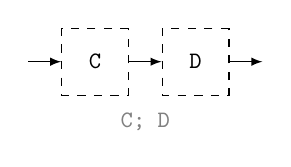
\begin{tikzpicture}[scale=0.85, transform shape]
  \node[proc] (C) at (0, 0) {C}; %
  \node[proc] (D) at ($(C)+(1.5, 0)$) {D};
  \draw[->] (-1, 0) -- (C);
  \draw[->] (C) -- (D);
  \draw[->] (D) -- ++(1, 0);

  \node[code] at ($(C)+(.75, -.9)$) {\texttt{C; D}};
\end{tikzpicture}\\[2pt] \small (a) Sequence\end{tabular}
\hfill
\begin{tabular}[b]{@{}c@{}}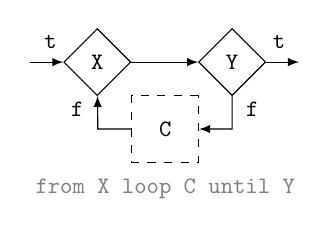
\begin{tikzpicture}[scale=0.85, transform shape]
  \node[assert] (X) at (0, 0) {X}; %
  \node[test, right=of X] (Y) {Y};
  \node[proc] (C) at ($(Y)+(-1, -1)$) {C};
  \draw[->] (-1, 0) -- (X);
  \node[label] at ($(X)+(-.7, .3)$) {t}; %
  \draw[->] (X) -- (Y);
  \draw[->] (Y) -- ++(1, 0);
  \node[label] at ($(Y)+(.7, .3)$) {t}; %
  \draw[->] (Y) -- ++(0,-1) -- ++(-0.4,0) -- (C);
  \node[label] at ($(Y)+(.3, -.7)$) {f}; %
  \draw[->] (C.west) -- ++(-.5, 0) coordinate (temp) -- (X);
  \node[label] at ($(X)+(-.3, -.7)$) {f};

  \node[code] at ($(C)+(0, -.9)$) {\texttt{from X loop C until Y}};
\end{tikzpicture}\\[2pt] \small (b) Reversible loop\end{tabular}
\hfill
\begin{tabular}[b]{@{}c@{}}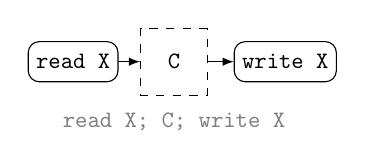
\begin{tikzpicture}[scale=0.85, transform shape]
  \node[terminal] (start) at (0,0) {\t{read X}};
  \node[proc,right=of start] (proc) at (0,0) {C};
  \node[terminal, right=of proc] (stop) at (1.4,0) {\t{write X}};

  \draw[->] (start) -- (proc);
  \draw[->] (proc) -- (stop);

  \node[code] at ($(proc)+(0, -.9)$) {\texttt{read X; C; write X}};
\end{tikzpicture}\\[2pt] \small (c) Structured terminals\end{tabular}
\end{document}
